\chapter{Fogos de Artifício}

\fontsize{12}{14}\selectfont


Os fogos de artifício têm uma história rica e fascinante que atravessa continentes e culturas, unindo ciência, arte e poder em uma única forma de expressão visual. Originários da China por volta do século IX, os fogos de artifício eram inicialmente utilizados como parte de rituais religiosos e cerimônias para espantar espíritos malignos e trazer boa sorte. Através das rotas comerciais e do contato cultural, a tecnologia dos fogos de artifício foi gradualmente introduzida na Europa durante o final da Idade Média e o início da Renascença, onde passaram a desempenhar um papel significativo em celebrações reais, religiosas e militares.

Na Europa moderna, os fogos de artifício rapidamente se tornaram uma forma de exibir poder e autoridade, especialmente por monarcas e figuras religiosas. Com seu poder de dominar o céu noturno, os fogos simbolizavam a capacidade dos governantes de controlar as forças da natureza, uma metáfora visual para sua autoridade política e espiritual. Além disso, o espetáculo proporcionado por explosões de luz e cor era uma forma de deslumbrar e impressionar as multidões, reforçando a imagem de grandiosidade e supremacia das instituições.

Entre os séculos XVI e XVIII, os fogos de artifício começaram a se transformar em espetáculos artísticos elaborados, especialmente nas cortes europeias. Reis e papas investiam em grandes exibições de fogos para marcar ocasiões especiais como coroações, casamentos, tratados de paz e vitórias militares. A tecnologia da pirotecnia avançou consideravelmente nesse período, com engenheiros e artesãos especializados no design de dispositivos cada vez mais complexos, capazes de criar formas e efeitos visuais mais sofisticados, como rodas de fogo, cascatas de luz e estruturas pirotécnicas de grande escala.

Além de seu uso em celebrações e festivais, os fogos de artifício também desempenhavam um papel simbólico na guerra. Eles foram adaptados como armas pirotécnicas em algumas situações, sendo usados tanto para fins de intimidação quanto para iluminar campos de batalha. No entanto, na maior parte do tempo, eles permaneciam como um símbolo de poder, riqueza e ordem, enaltecendo o prestígio dos governantes e suas cortes.

O contexto religioso não era menos significativo. Na Itália, especialmente em Roma, fogos de artifício como La Girandola se tornaram uma tradição anual. Essas exibições eram realizadas em datas importantes do calendário católico, como a Festa dos Santos Pedro e Paulo, e serviam como um meio de reafirmar o poder da Igreja Católica, combinando um
espetáculo visual grandioso com o reforço da autoridade papal.

Culturalmente, os fogos de artifício também eram vistos como uma manifestação do sublime, um conceito estético que descreve a experiência de ser sobrecarregado por algo vasto, belo e ao mesmo tempo aterrorizante. Filósofos como Edmund Burke, no século XVIII, discutiram como o poder de algo como os fogos de artifício, ao provocar tanto fascínio quanto medo, capturava a essência do sublime. Através desse prisma, as exibições pirotécnicas não eram apenas entretenimento; eram uma experiência que tocava no mais profundo da psique humana, evocando emoções intensas e duradouras.

Em termos artísticos, os fogos de artifício influenciaram uma vasta gama de representações visuais, especialmente em gravuras e pinturas da época. Muitos artistas buscavam capturar a efemeridade e o dinamismo desses espetáculos em suas obras, desafiando as limitações do papel e da tinta para transmitir a luz e o movimento dos fogos. Essas representações artísticas se tornaram uma forma de preservar a memória de grandes celebrações e eventos, permitindo que o público revivesse essas experiências visuais por gerações.

Assim, os fogos de artifício, desde sua invenção até sua disseminação na Europa moderna, evoluíram de meros explosivos cerimoniais para uma forma altamente refinada de arte pública e propaganda política. Eles combinavam ciência e espetáculo, expressando a busca humana por controle sobre as forças naturais enquanto proporcionavam um espetáculo visual que fascinava tanto os reis quanto seus súditos. Ao longo dos séculos, os fogos de artifício continuaram a ser uma ferramenta poderosa de celebração, uma forma de arte efêmera e uma demonstração do progresso técnico e artístico da humanidade.

La Girandola foi uma das exibições de fogos de artifício mais icônicas de Roma, simbolizando a combinação de esplendor visual com o poder espiritual e temporal. Originada no século XVI, essa apresentação pirotécnica se tornou uma tradição anual associada a importantes festividades, como a celebração dos Santos Pedro e Paulo, padroeiros de Roma, e outros grandes eventos religiosos e políticos. Sua realização era uma forma de a Igreja Católica reafirmar sua autoridade sobre o povo e exibir seu papel central na vida pública da cidade.

\begin{figure}[htbp]
  \centering
  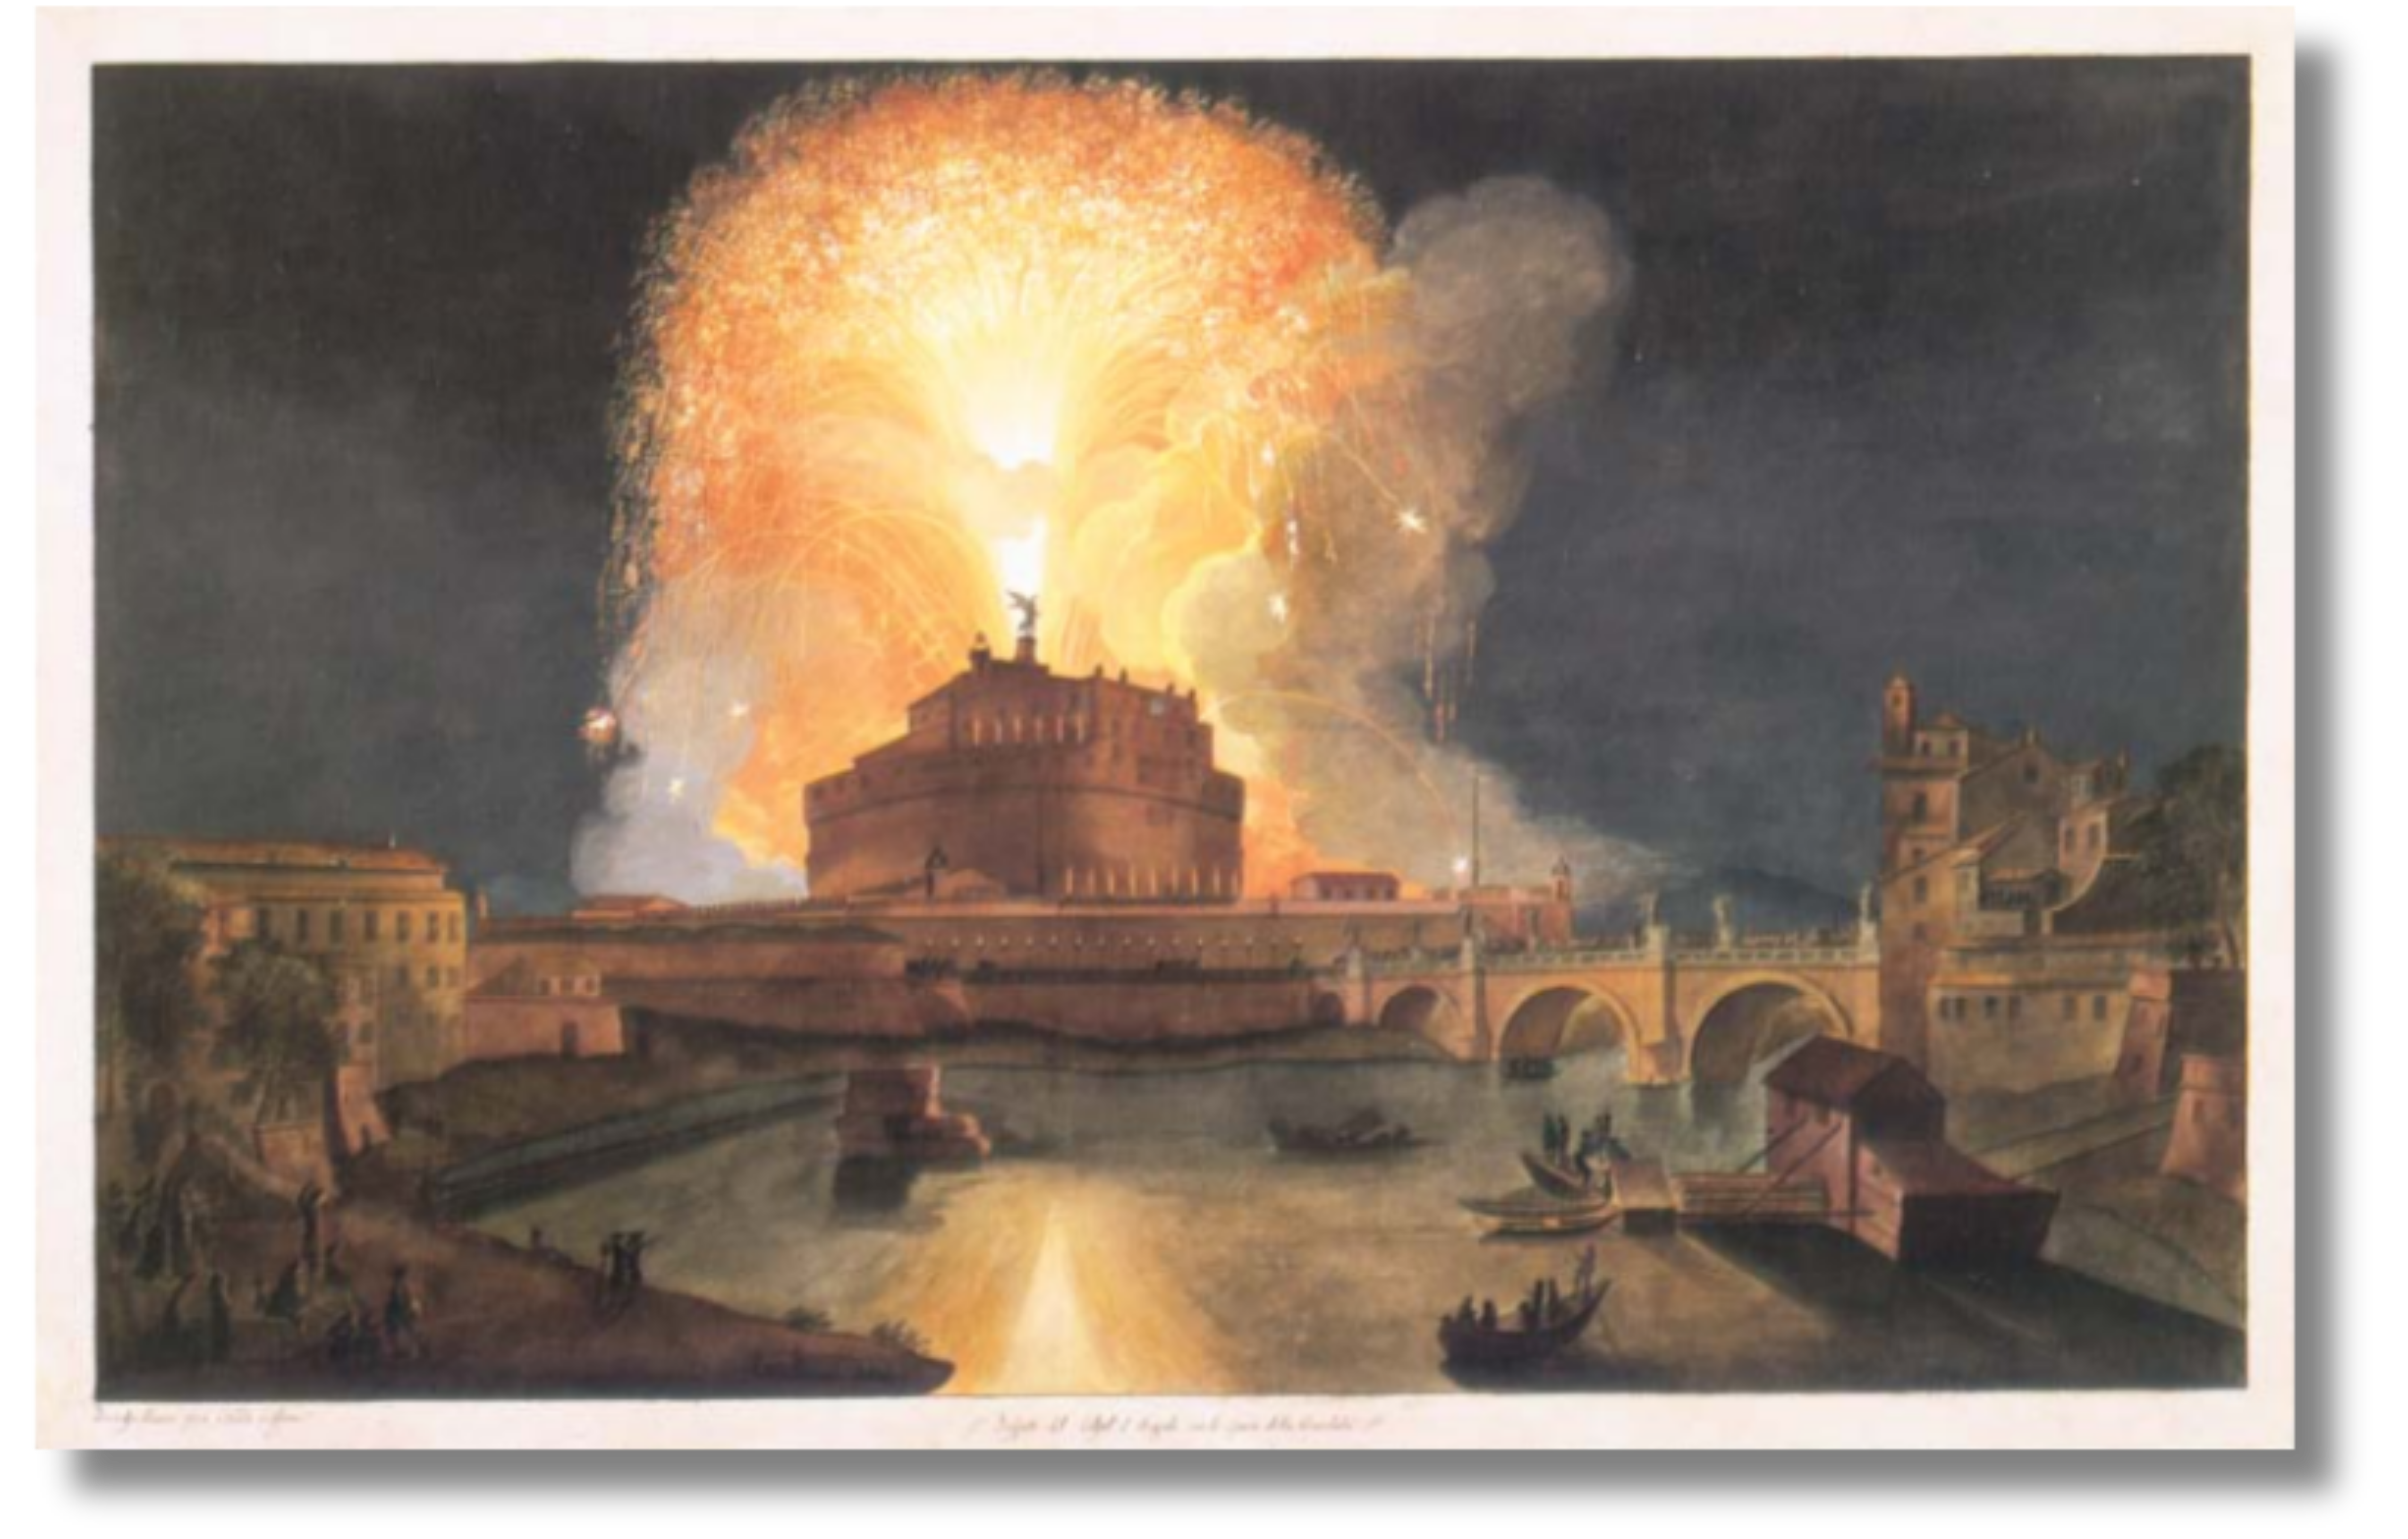
\includegraphics[width=0.8\textwidth]{Castel Sant'Angelo, Rome, with the Girandola.png}
  \caption{\fontsize{8}{8}\selectfont \textbf{Francesco Panini} (1745 - 1812) II prospetto del Castel' St. Angiolo con lo sparo della Girandola Castel Sant'Angelo, Rome, with the Girandola Hand-colored (watercolor and gouche) etching. 22(7/8) x 34(7/8) in (58.0 x 88.6 cm)}
  \label{fig:Castel_sant_angelo}
\end{figure}

A gravura intitulada II Prospetto del Castel' St. Angiolo con lo Spara della Girandola, criada por Francesco Panini (1745-1812), é uma obra que captura o espetáculo dos fogos de artifício que emanavam do Castel Sant'Angelo, um monumento historicamente carregado de simbolismo. O Castel Sant'Angelo, originalmente construído como um mausoléu para o imperador Adriano, foi transformado ao longo dos séculos em uma fortaleza papal, servindo como refúgio seguro para os papas e também como prisão. O local, estrategicamente posicionado nas margens do rio Tibre, proporcionava o cenário perfeito para a impressionante exibição da Girandola.

Panini, um mestre das paisagens arquitetônicas e urbanas, retrata a explosão de fogos de artifício com uma técnica de gravura meticulosamente detalhada, colorida à mão com aquarela e guache. A obra é caracterizada pela precisão na captura das luzes dos fogos refletidas na água e pelos delicados detalhes das multidões que se reuniam para assistir ao espetáculo. As colunas de fumaça ascendendo ao céu noturno, iluminado pelas explosões, são compostas de forma quase teatral, enfatizando a grandiosidade e o controle da Igreja sobre o fogo, um elemento que sempre carregou significados profundos.

No contexto histórico, La Girandola surgiu em uma época em que a Igreja Católica buscava reafirmar sua supremacia após períodos de contestação, como a Reforma Protestante no século XVI e as Guerras Religiosas. Os espetáculos pirotécnicos, que reuniam multidões de fiéis e dignitários estrangeiros, eram utilizados para mostrar que a Igreja não só sobrevivera a essas crises, como também permanecia poderosa e central na vida europeia. A forma circular dos fogos, que na Girandola imitava a coroa papal, sugeria a continuidade e a eternidade da autoridade papal.

\begin{wrapfigure}{r}{0.4\textwidth} % Posição (r = direita), largura da imagem
    \centering
    \includegraphics[width=\linewidth]{The Girándola over Castel Sant'Angelo.png}
    \caption{\fontsize{8}{8}\selectfont \textbf{Francesco Piranesi} (1756-1810), etcher  Lou is-Jean Desprez (1743-1804), watercolorist The Girándola over Castel Sant'Angelo [Rome?: n.p., ca. 1783] Hand-colored (watercolor and gouache) etching. 26 5/8 x 18 1/8 in (67.6 x 46.4 cm) }
\end{wrapfigure}

A precisão coreografada da exibição pirotécnica refletia a ordem e a disciplina impostas pela Igreja, contrastando com o caos inerente do fogo. Este controle da destruição e da luz funcionava como uma metáfora visual da capacidade da Igreja de domar as forças naturais e espirituais, trazendo ordem ao caos do mundo. Não era apenas uma demonstração de entretenimento, mas um poderoso exercício de propaganda, reforçando a ideia de que o papado estava no centro de todas as coisas, tanto no plano terreno quanto no celestial.

Além disso, a obra de Panini também revela aspectos importantes da vida social de Roma no período Barroco e Neoclássico. As multidões retratadas na gravura são um testemunho do fascínio popular por esses espetáculos públicos. Fogos de artifício, embora efêmeros, tinham um impacto duradouro na memória coletiva e eram um meio eficaz de envolver tanto as elites quanto o povo comum nas celebrações oficiais. A grandiosidade da Girandola proporcionava um sentimento de pertencimento ao vasto império espiritual da Igreja, reafirmando a posição de Roma como o coração da Cristandade.

O uso de fogos de artifício na Europa moderna também era visto como uma forma de exibição do domínio tecnológico, mostrando o avanço das técnicas de pirotecnia e a habilidade dos artesãos. A coordenação necessária para executar uma Girandola de forma precisa envolvia planejamento militar, engenheiros habilidosos e um profundo conhecimento dos materiais combustíveis. Esta exibição de domínio sobre as forças da natureza servia para comunicar ao público que a ordem estabelecida pela Igreja e pelo Estado era inquebrantável, uma vez que até o fogo, símbolo de destruição e renovação, estava sob seu controle.

\begin{wrapfigure}{r}{0.4\textwidth} % Posição (r = direita), largura da imagem
    \centering
    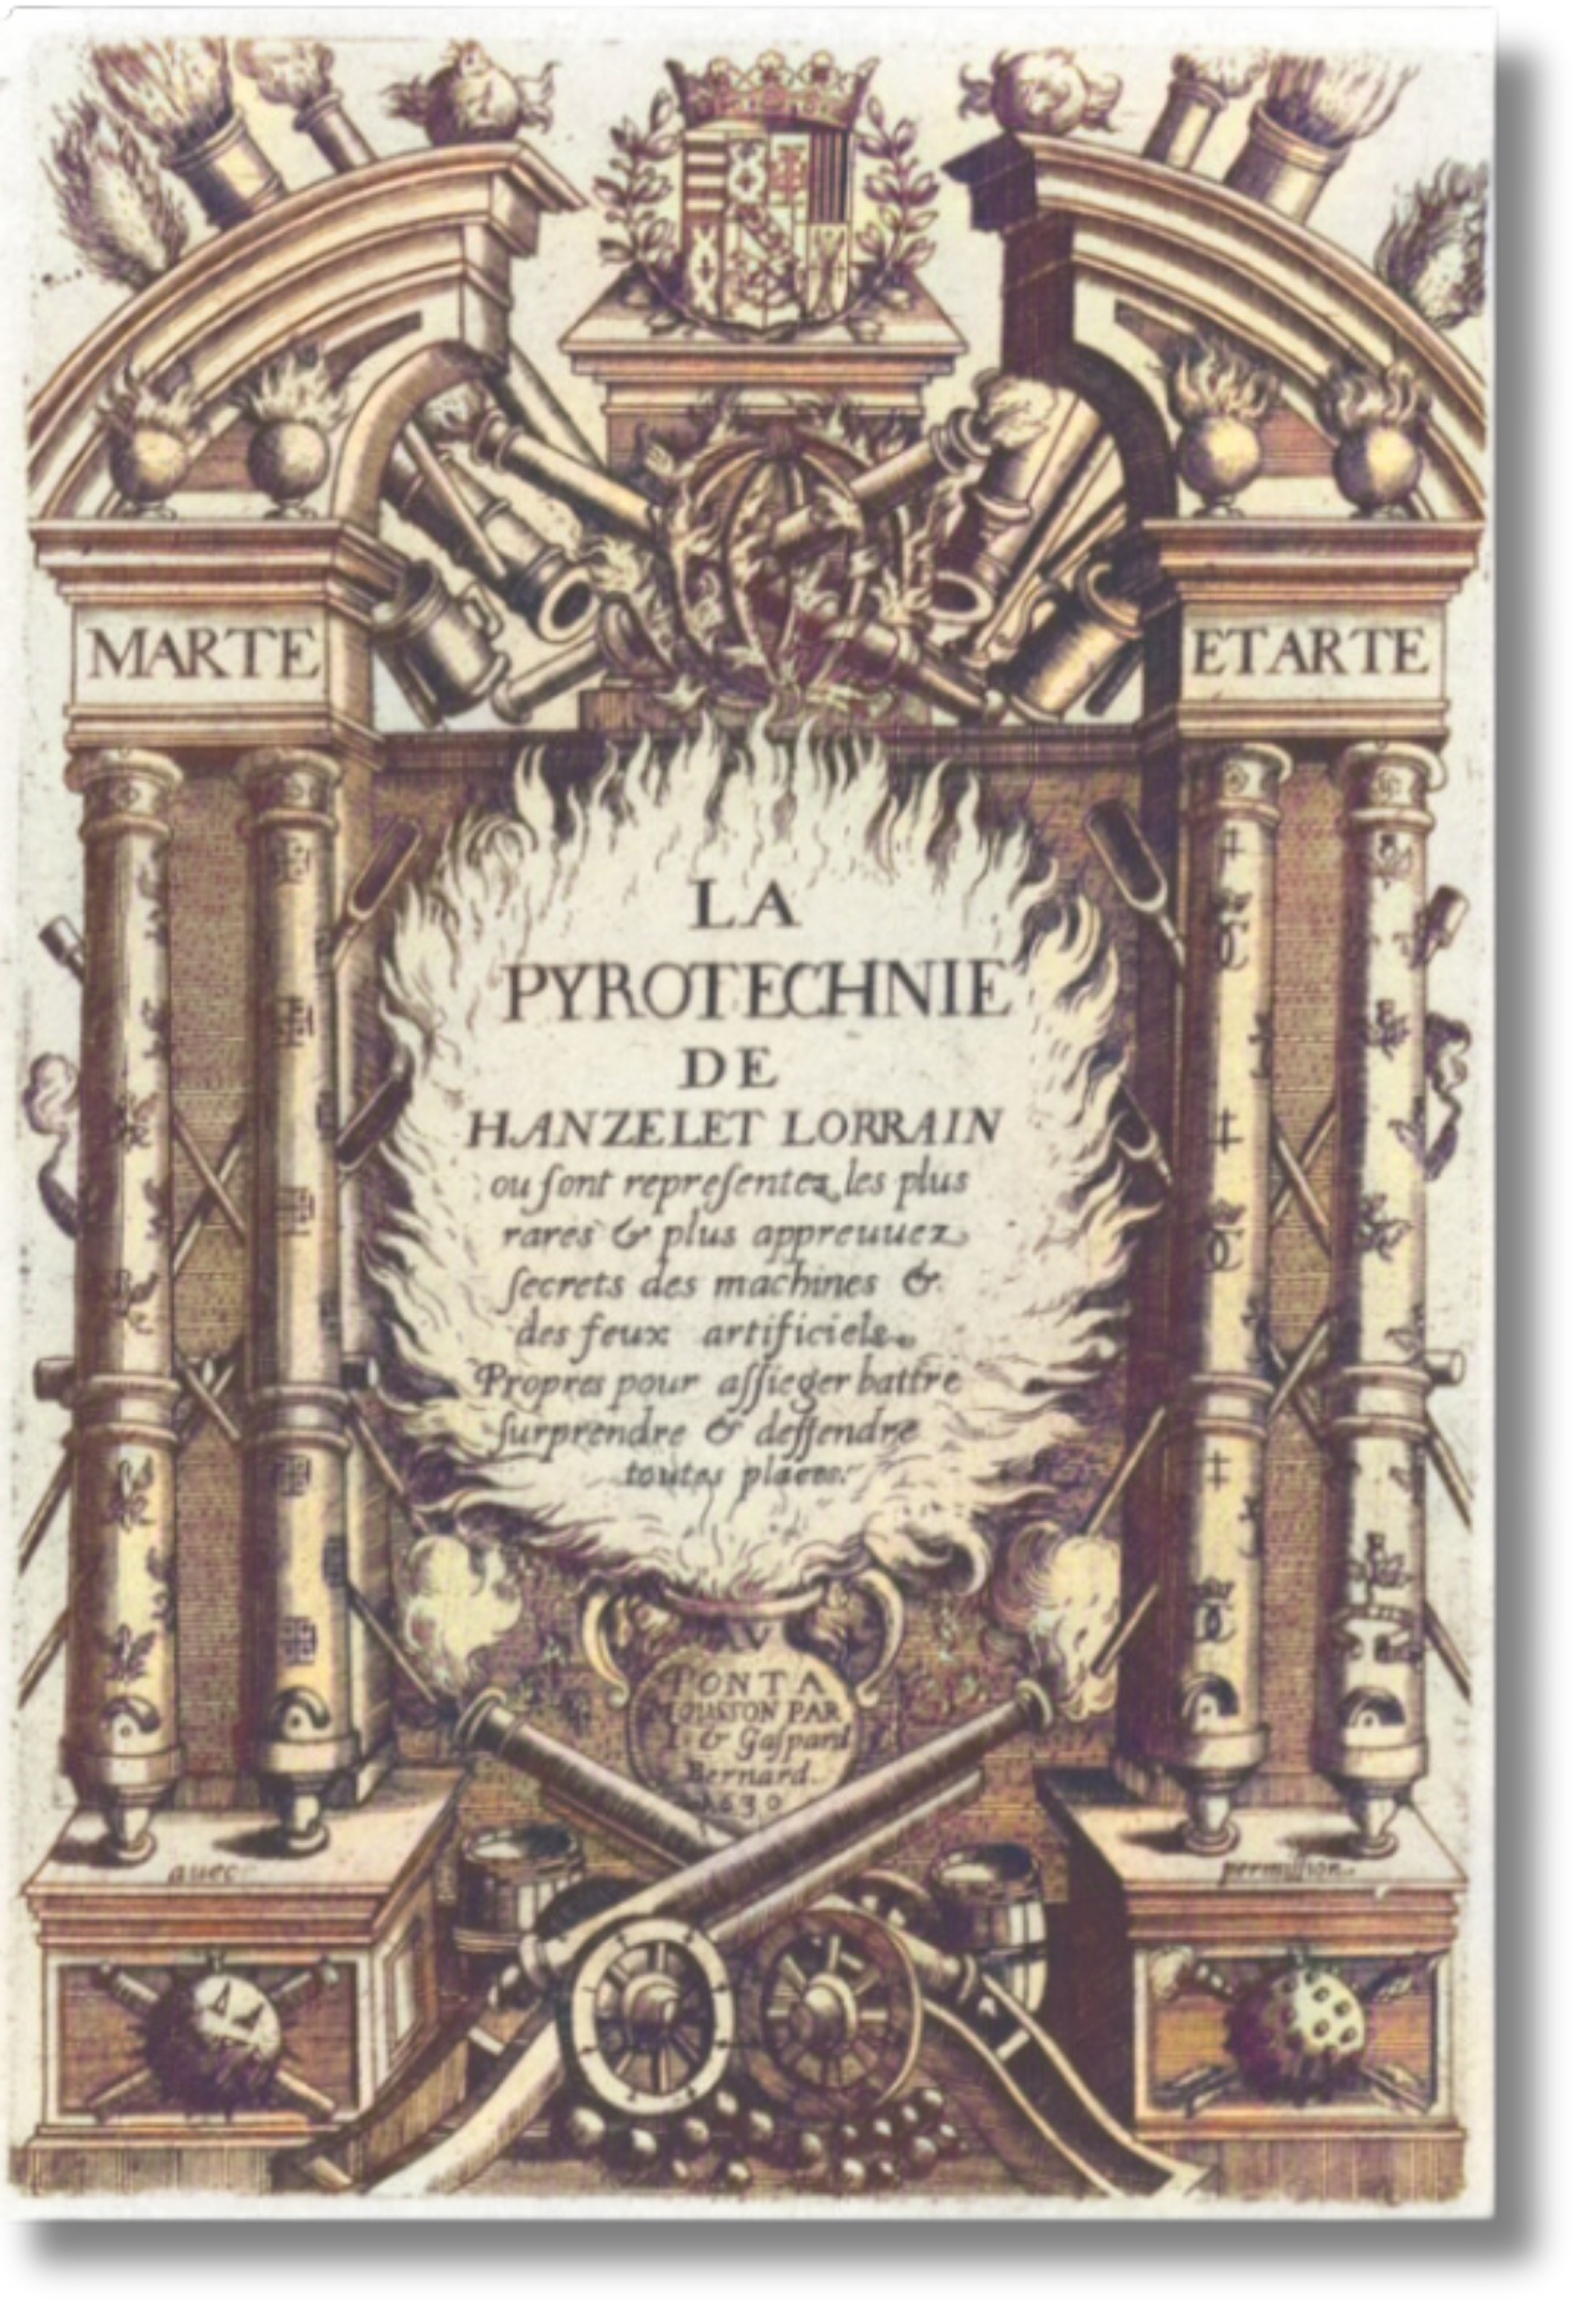
\includegraphics[width=\linewidth]{Title Page.png}
    \caption{\fontsize{8}{8}\selectfont \textbf{Anonymous} Title Page Engraving. 9(1/4) x 6(1/2) in (23.5 x 16.5 cm) From: Appier Hanzelet, Pyrotechnie (1630) }
\end{wrapfigure}

Publicado em 1630, La Pyrotechnie de Jean Appier Hanzelet é um dos primeiros tratados europeus sobre a arte dos fogos de artifício. O livro é um compêndio de técnicas pirotécnicas, diagramas de dispositivos e explicações detalhadas sobre a produção e o uso de fogos de artifício tanto em celebrações quanto em combates militares. A obra reflete o crescente interesse pelo controle científico dos elementos e o desejo de domar o fogo para criar espetáculos ordenados e impressionantes. La Pyrotechnie serviu como um manual para engenheiros e artistas, unindo ciência e arte em uma era em que o controle sobre o fogo era visto como um símbolo de poder e inovação.

\begin{wrapfigure}{r}{0.4\textwidth} % Posição (r = direita), largura da imagem
    \centering
    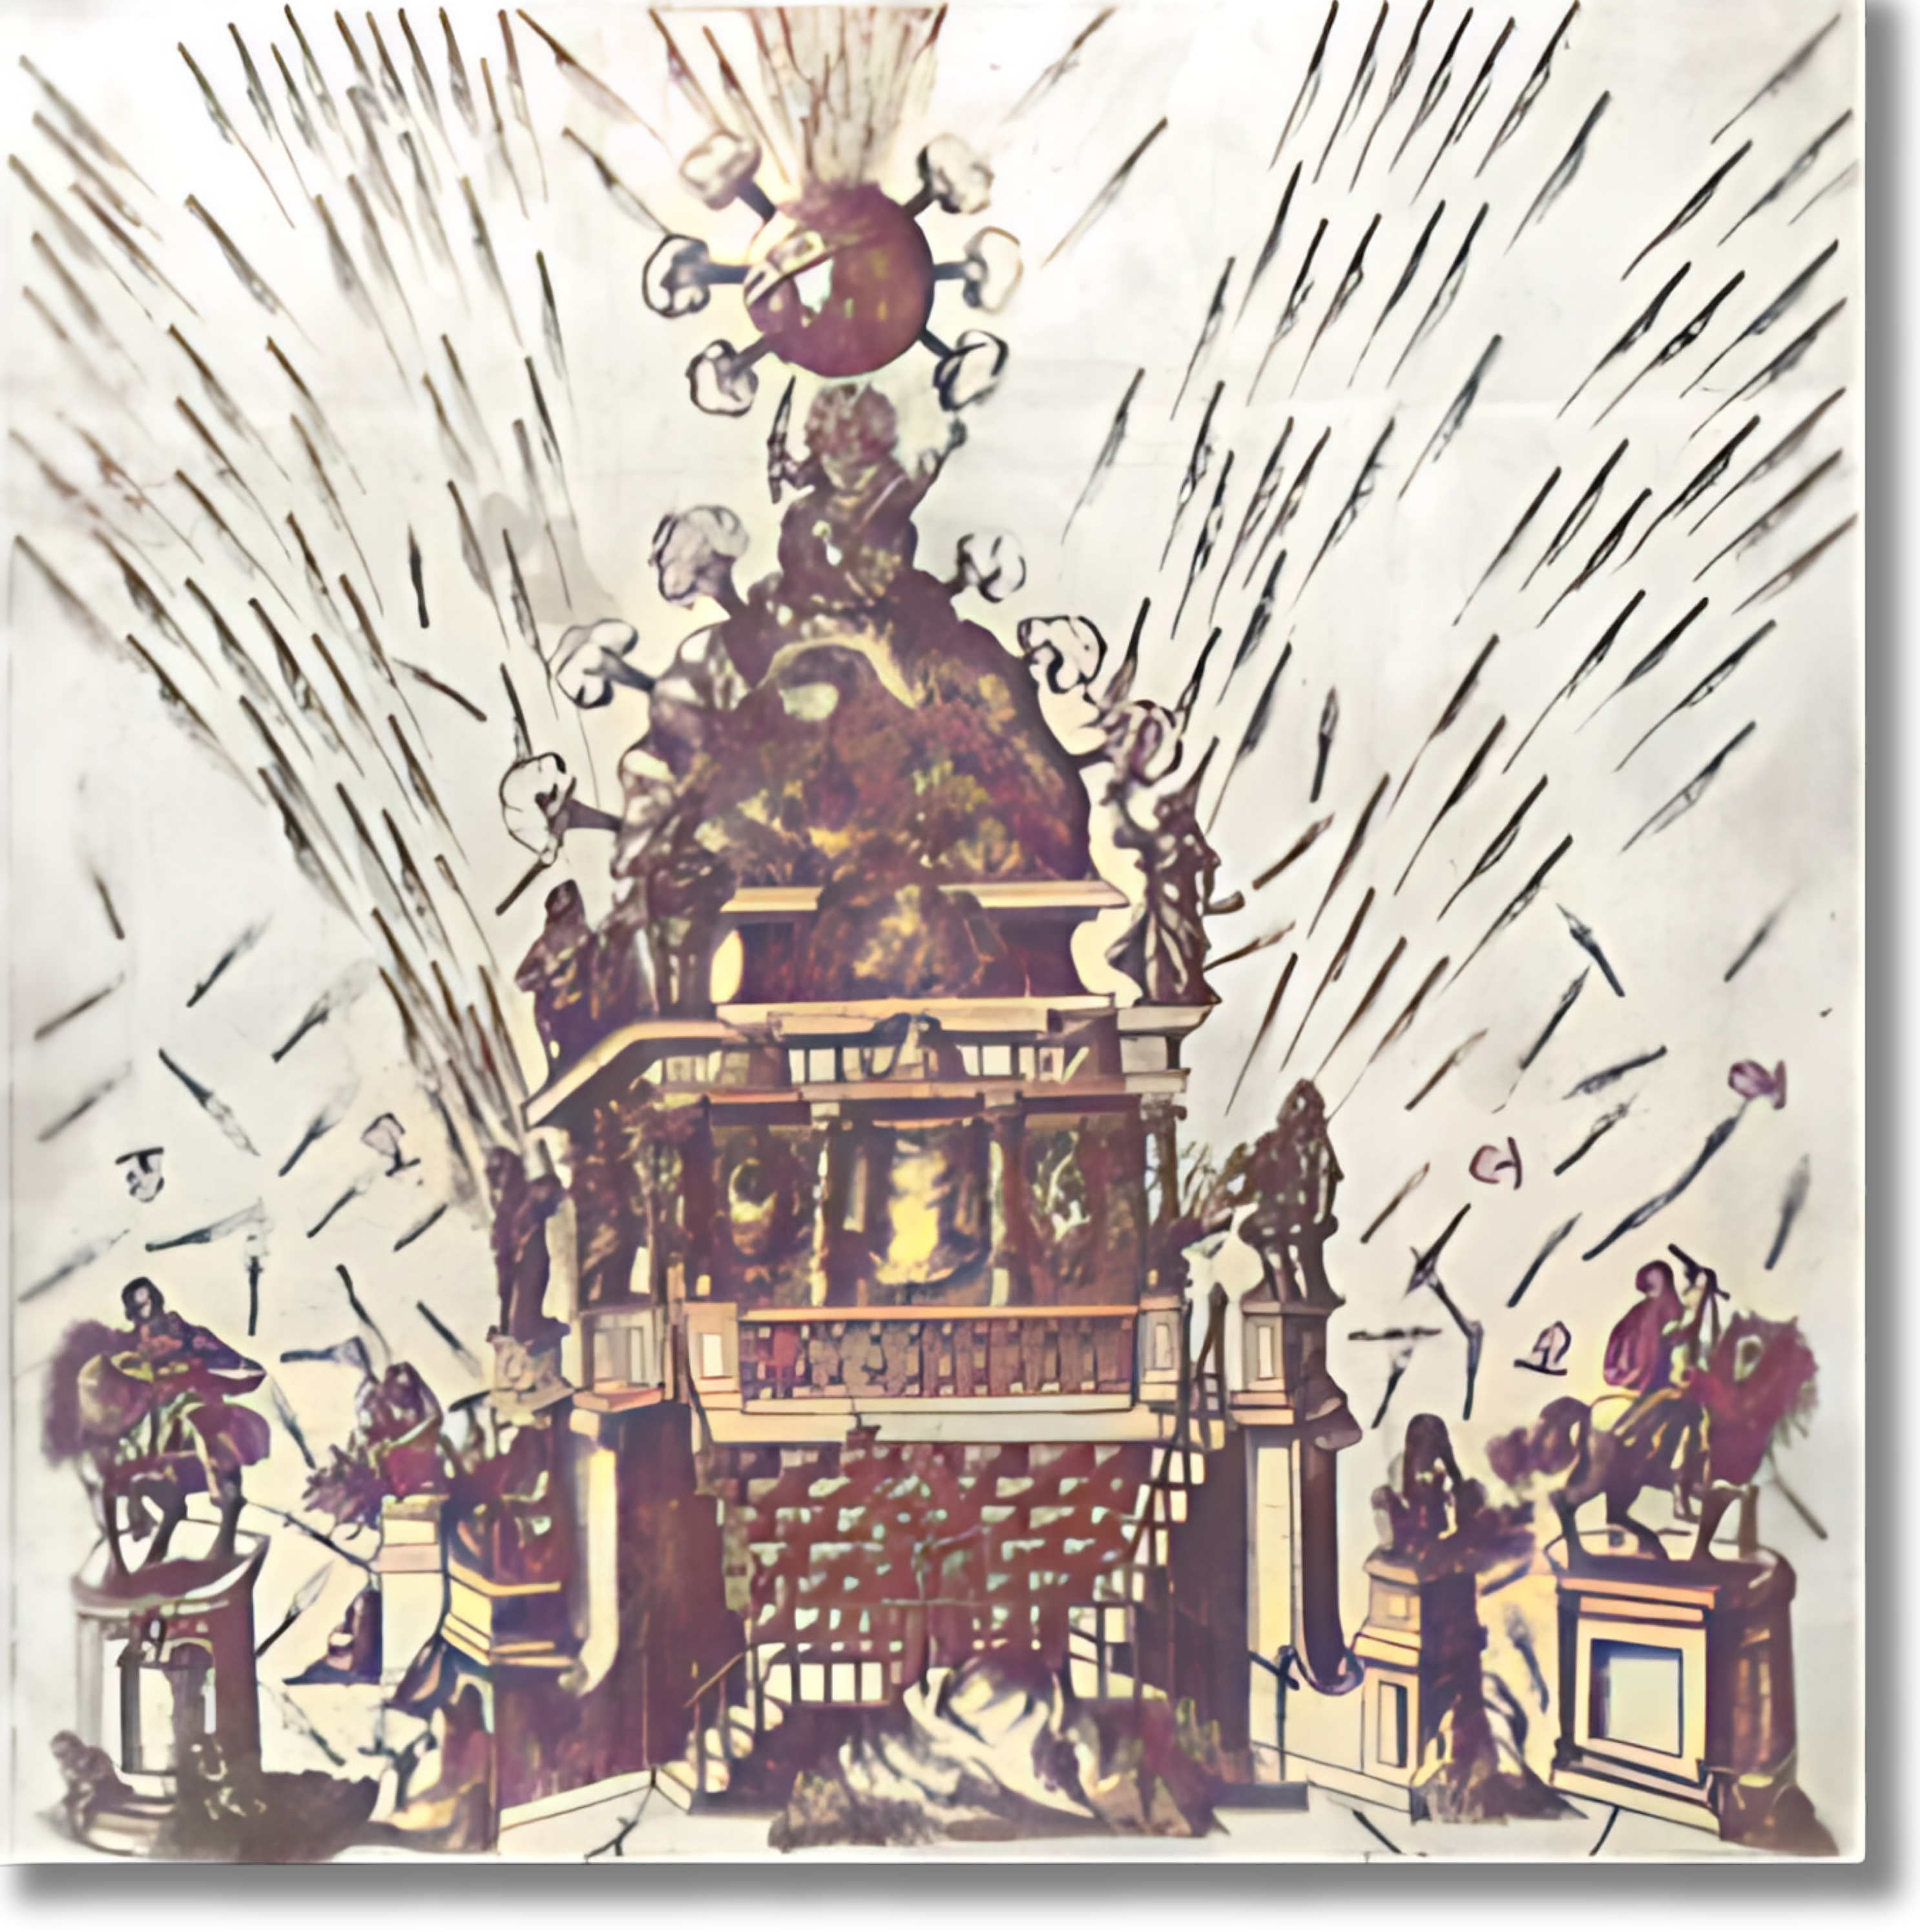
\includegraphics[width=\linewidth]{Fireworks machine in the shape of Mount Parnassus.png}
    \caption{\fontsize{8}{8}\selectfont \textbf{F.M.R. [?], etcher} Fireworks machine in the shape of Mount Parnassus Etching. 14(3/4) x 12(5/8) in (37.5 x 32.0 cm) From: Boscoli, Applausi (1658) }
\end{wrapfigure}

Em 1658, uma máquina de fogos de artifício foi construída em forma de Monte Parnaso, uma referência mitológica à morada das Musas e símbolo do conhecimento e da arte. Este tipo de estrutura complexa e alegórica era comum em celebrações barrocas, onde os fogos de artifício não apenas entretinham, mas também transmitiam mensagens simbólicas. O Monte Parnaso, nesse contexto, representava a elevação espiritual e intelectual proporcionada pela monarquia e a corte, sugerindo que o poder real era iluminado pelo conhecimento e pela inspiração divina. Esta gravura detalha a máquina com fogos irradiando de sua base e do topo, simbolizando o esplendor e a majestade do evento.

\begin{wrapfigure}{r}{0.4\textwidth}[h] % Posição (r = direita), largura da imagem
    \centering
    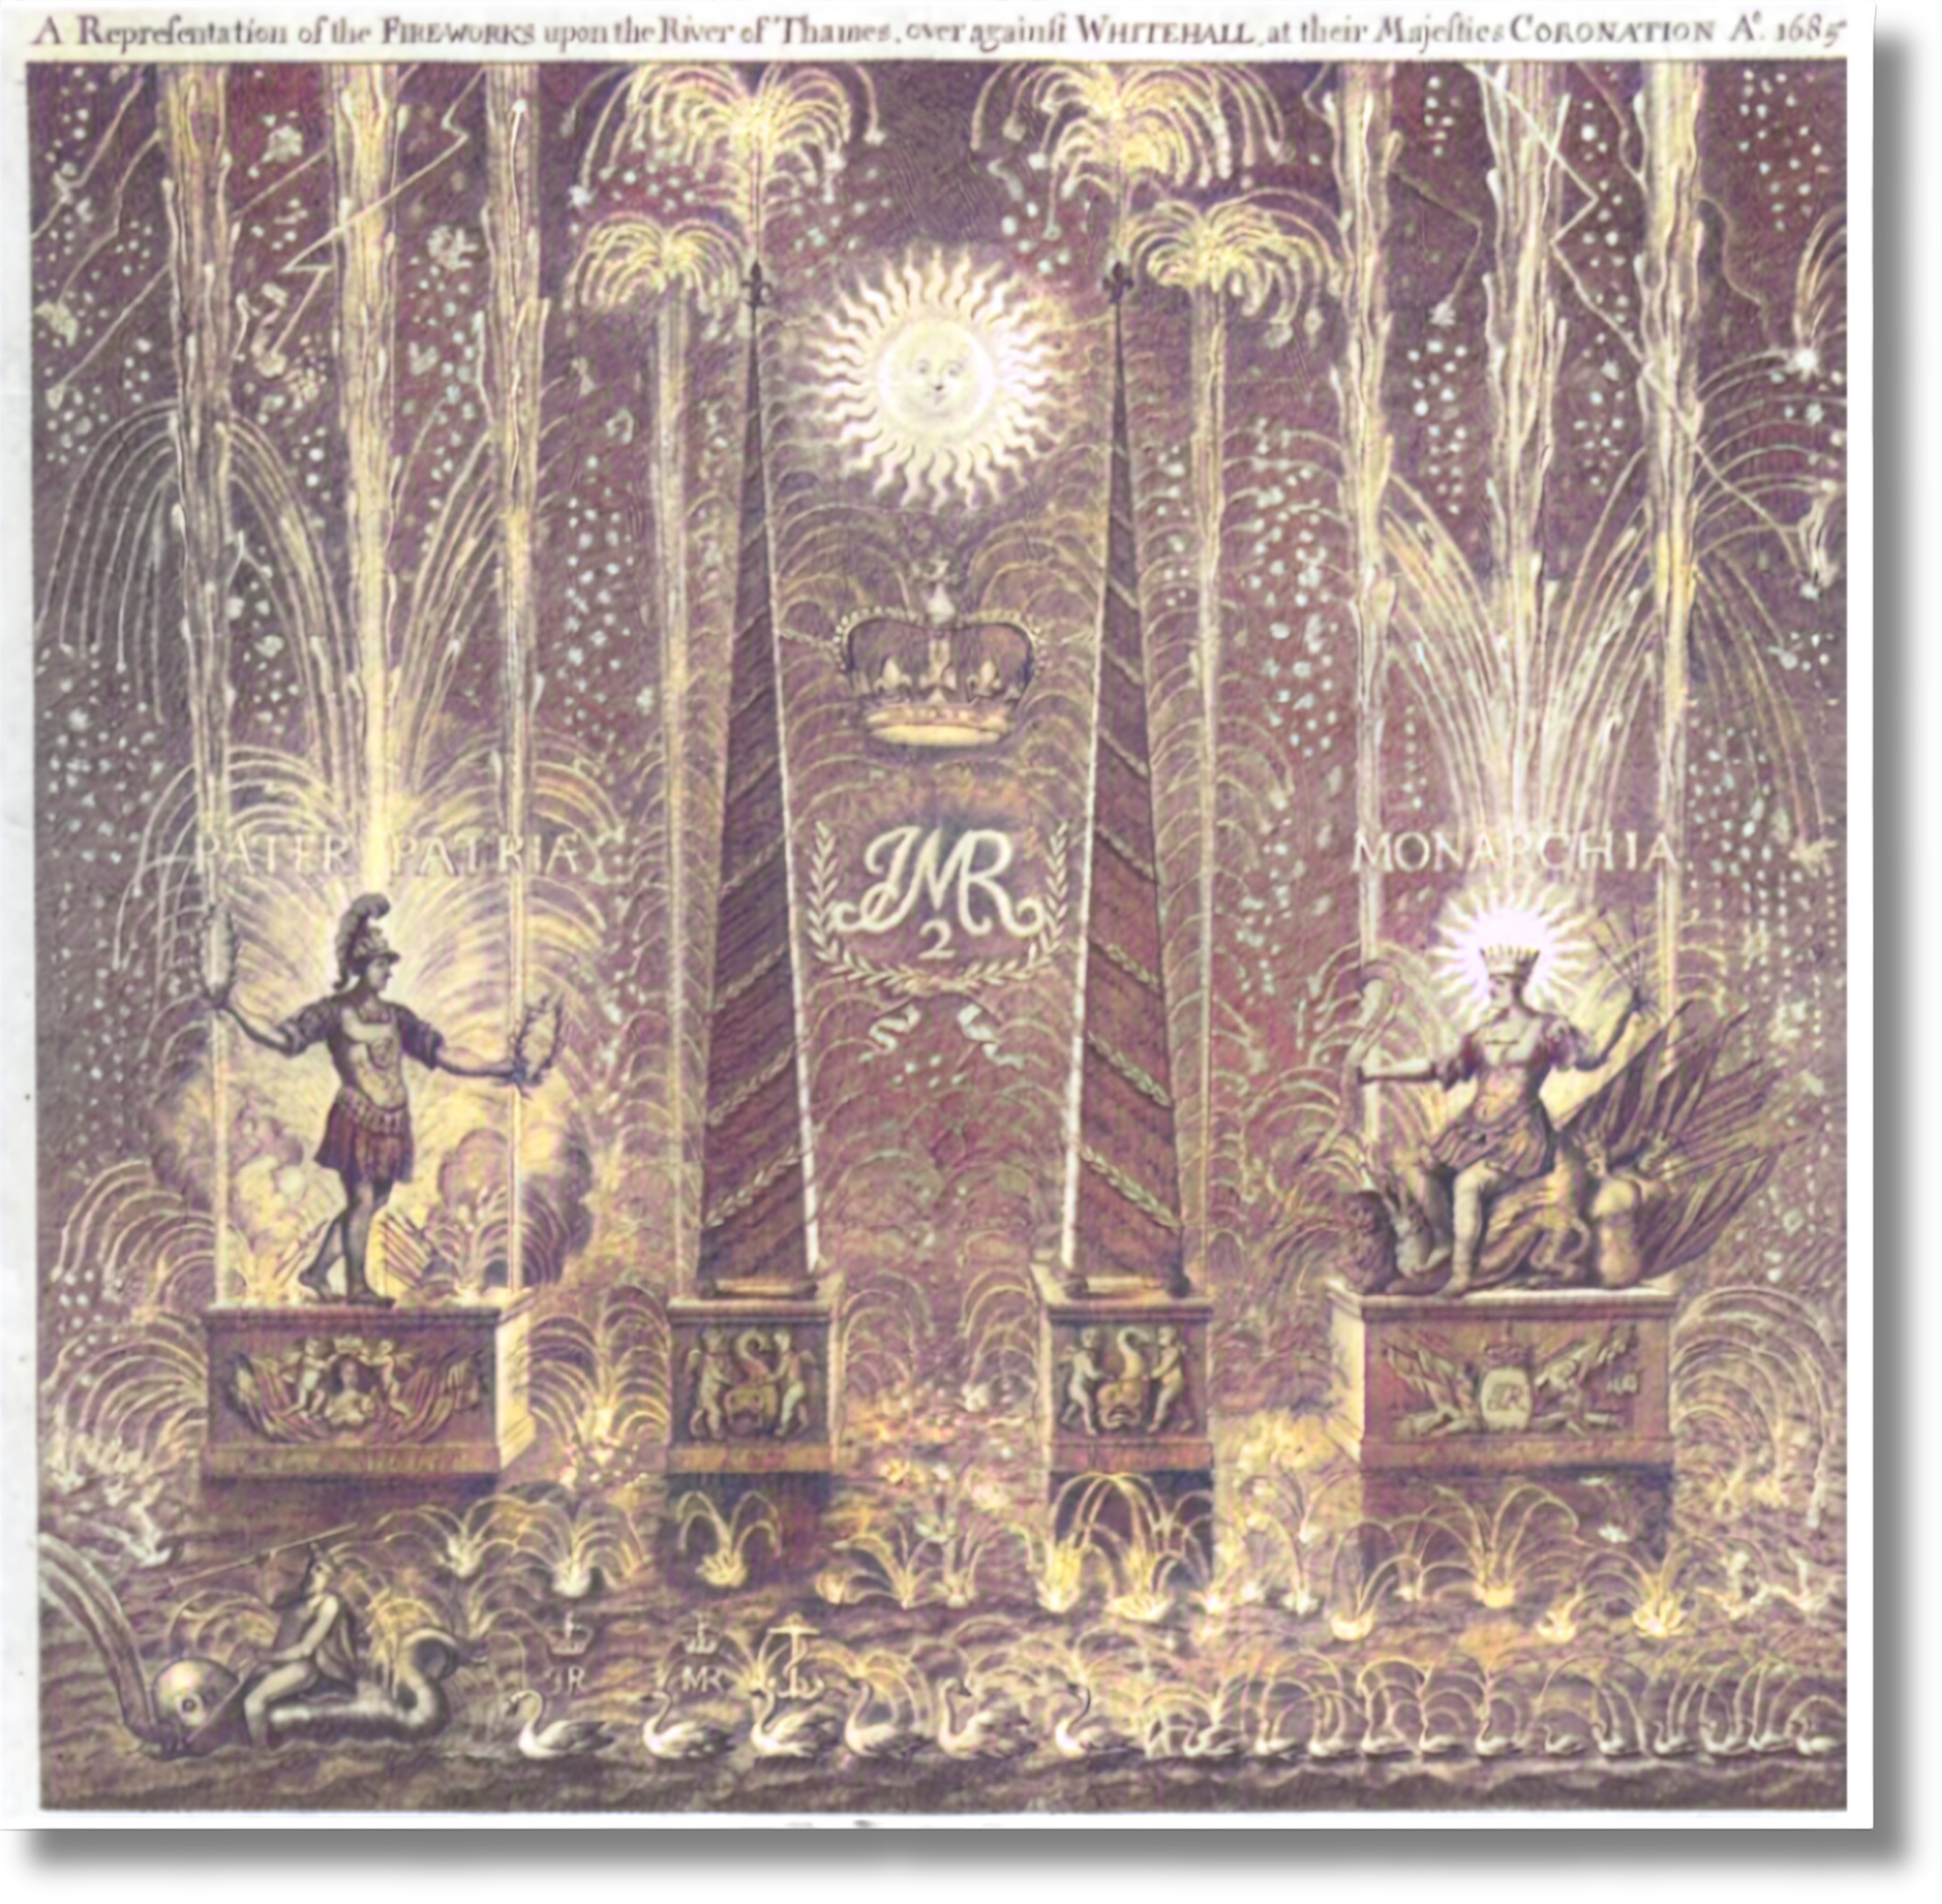
\includegraphics[width=\linewidth]{A representation of the fire-works upon the river of Thames, over against Whitehall, at their majesties coronation.png}
    \caption{\fontsize{8}{8}\selectfont \textbf{Anonymous} A representation of the fire-works upon the river of Thames, over against Whitehall, at their majesties coronation A°. 1685 Fireworks for the coronation of James II [London: n.p., 1685?] Engraving. 17 3/8 x 205/8 in (44.0 x 52.3 cm) GRI, Brock Fireworks Collection, acc. no. P950001**-019 }
\end{wrapfigure}

A coroação de James II da Inglaterra em 1685 foi marcada por uma das mais grandiosas exibições de fogos de artifício do período. Realizada sobre o rio Tâmisa, esta exibição simbolizava o poder e a continuidade da monarquia inglesa. Os fogos de artifício, lançados de barcaças no rio, eram cuidadosamente coreografados para criar imagens no céu, como coroas e escudos, reforçando o tema da realeza e do direito divino dos reis. Esta gravura documenta o evento, mostrando o rio iluminado e as multidões nas margens, impressionadas pelo espetáculo de luzes e som que celebrava a ascensão de James II ao trono.

\begin{wrapfigure}{r}{0.4\textwidth} % Posição (r = direita), largura da imagem
    \centering
    \includegraphics[width=\linewidth]{Feu d'artifice exécuté le 25 aoust 1777.png}
    \caption{\fontsize{8}{8}\selectfont \textbf{Lorenz Ludwíg Midart (1733-1800), draftsman Christian von Mechel (1737-1817), engraver?} Feu d'artifice exécuté le 25 aoust 1777. sur le glacis de la ville de Soleure... à l'occasion du renouvellementd'alliance entre l'auguste couronne de France et le louable corps helvétique Fireworks held on 25 August 1777 in Soleure, Switzerland, for the renewal of the alliance between France and Switzerland Basel: Christian von Mechel, 1779 Engraving. 14 1/8 x 17 5/8 in (35.8 x 44.6 cm) }
\end{wrapfigure}

Em 1777, Soleure, na Suíça, foi o cenário de uma celebração pirotécnica grandiosa para marcar a renovação da aliança entre a França e a Suíça. Este evento, que ocorreu em uma época de intensa diplomacia europeia, foi um exemplo clássico de como os fogos de artifício eram usados para simbolizar a união e o poder entre nações. A gravura de Lorenz Ludwig Midart retrata a exibição com atenção aos detalhes, mostrando as multidões reunidas e os fogos iluminando a cidade. As explosões de fogos no céu, refletidas na água do rio Aar, capturam a atmosfera de celebração e a importância simbólica da ocasião.